% to get the standard slides
% \documentclass[xcolor=x11names]{beamer}
% \usetheme{Boadilla}

% to get the handout
\documentclass[xcolor=x11names,handout]{beamer}
\usepackage{pgfpages}
\pgfpagesuselayout{4 on 1}[a4paper,landscape, border shrink=5mm]
\pgfpageslogicalpageoptions{1}{border code=\pgfusepath{stroke}}
\pgfpageslogicalpageoptions{2}{border code=\pgfusepath{stroke}}
\pgfpageslogicalpageoptions{3}{border code=\pgfusepath{stroke}}
\pgfpageslogicalpageoptions{4}{border code=\pgfusepath{stroke}}
\usetheme{default}

%\bibliographystyle{chicago}
%\bibpunct[]{(}{)}{,}{a}{}{,}
\usepackage{multirow}
\usepackage{tabularx}
\usepackage{array}
% \usepackage{pifont}
\usepackage{graphics}
\usepackage{xcolor}
\usepackage{hyperref}
\usepackage[utf8]{inputenc}
\usepackage{pifont}% http://ctan.org/pkg/pifont
\usepackage{natbib}
\usepackage{amsmath}

\usepackage[makeroom]{cancel}

\usepackage{pythonhighlight}
\usepackage{fontawesome}

\newcommand{\light}[1]{\textcolor{gray}{#1}}
\newcommand{\cmark}{\ding{51}}%
\newcommand{\xmark}{\ding{55}}%
\newcolumntype{C}[1]{>{\centering\let\newline\\\arraybackslash\hspace{0pt}}m{#1}
}

\usetheme{UNIBO}

\newcommand{\btVFill}{\vskip0pt plus 1filll}

\newcommand{\yellow}[1]{\textcolor{yellow}{#1}}
\newcommand{\red}[1]{\textcolor{red}{#1}}
\newcommand{\orange}[1]{\textcolor{orange}{#1}}


\newcommand*{\vcenteredhbox}[1]{\begingroup
	\setbox0=\hbox{#1}\parbox{\wd0}{\box0}\endgroup}

\DeclareRobustCommand{\rchi}{{\mathpalette\irchi\relax}}
\newcommand{\irchi}[2]{\raisebox{\depth}{$#1\chi$}}

\DeclareMathOperator*{\argmax}{arg\,max}

\makeatletter
\setbeamertemplate{footline}
{%
	\leavevmode%
	\hbox{%

\begin{beamercolorbox}[wd=.333333\paperwidth,ht=2.25ex,dp=1ex,center]{author in
head/foot}%
			\usebeamerfont{author in
head/foot}\insertshortauthor%
% ~~\beamer@ifempty{\insertshortinstitute}{}{(\insertshortinstitute)}
		\end{beamercolorbox}%

\begin{beamercolorbox}[wd=.333333\paperwidth,ht=2.25ex,dp=1ex,center]{title in
head/foot}%
			\usebeamerfont{title in head/foot}\insertshorttitle
		\end{beamercolorbox}%

\begin{beamercolorbox}[wd=.333333\paperwidth,ht=2.25ex,dp=1ex,right]{date in
head/foot}%
			\usebeamerfont{date in head/foot}\insertshortdate{}\hspace*{2em}
			\insertframenumber{} / \inserttotalframenumber\hspace*{2ex}
		\end{beamercolorbox}}%
	}
	\makeatother

\title[DIT, PhD]{\vspace{-2pt}\\
\href{http://www.dit.unibo.it}{
\includegraphics[width=30mm]{img/UNIBO_logo.png}
} \\
\vspace{6mm} {DIT PhD\\ Introduction to Computational Thinking and Programming} 
\\
{\large Lesson 3. Python 4 Poets}
% \\
% v 2.3 (PhD) January--February 2024
\vspace{-5mm}}

\author[A. Barr\'on-Cede\~no]{{Alberto Barr\'on-Cede\~no \\ a.barron@unibo.it
\vspace{-8mm}}
\institute[DIT-UniBO]{DIT-UniBO}}
\date[2024]{12/11/2024}

\let\Tiny=\tiny

\begin{document}

{%
\usebackgroundtemplate{%
	
\includegraphics[width=\paperwidth,
	height=\paperheight]{background.png} }
	\begin{frame}[plain]
		\titlepage
	\end{frame}
}

\begin{frame}
\frametitle{Programming}
\vspace{5mm}

\begin{center}
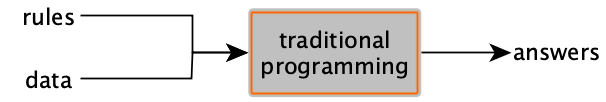
\includegraphics[width=100mm]{img/coli2020_diagrams_traditional_programming.png}
\end{center}

\btVFill
\footnotesize
\light{Diagram borrowed from L. Moroney's Introduction to TensorFlow for Artificial Intelligence, Machine Learning, and Deep Learning}
\end{frame}

\begin{frame}
\frametitle{Conditionals and Loops}
\vspace{5mm}

\begin{columns}
\begin{column}{0.4\textwidth}
 \begin{center}
 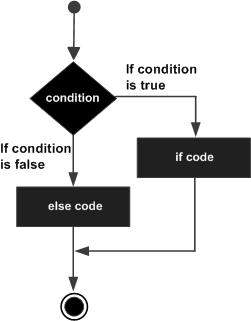
\includegraphics[width=4cm]{img/if_else_statement.jpg}
\end{center}
\end{column}					\pause 
\begin{column}{0.4\textwidth}
 \begin{center}
 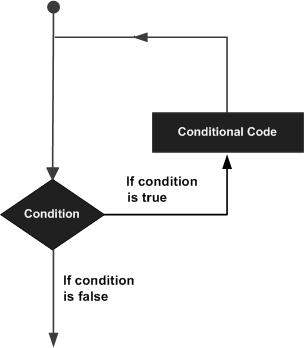
\includegraphics[width=4cm]{img/loop_architecture.jpg}
\end{center}
\end{column}
\end{columns}

\btVFill
\onslide
\footnotesize
\light{Diagrams borrowed from \url{https://www.tutorialspoint.com}}
\end{frame}

\begin{frame}[fragile]
\frametitle{Functions (methods)}

\textbf{A simple function}
\begin{python}
  def name_of_the_function(input1, input2):
      # function code
      none
\end{python}
\pause

\textbf{Calling the function}
\begin{python}
name_of_the_function("hi", "ho")
\end{python}
\pause

\textbf{Another valid call}
\begin{python}
name_of_the_function(hi, ho)
\end{python}
\pause

\textbf{An invalid call}
\begin{python}
name_of_the_function(hi)
\end{python}
\end{frame}

\begin{frame}
\frametitle{From Unix to Python}

\begin{itemize}
  \item Kenneth W.\ Church's \alert{Unix for poets}%
\footnote{\url{https://web.stanford.edu/class/cs124/kwc-unix-for-poets.pdf}}
\end{itemize}
\medskip            \pause

\centering

$\downarrow$
\medskip

\alert{Python for Poets}
\end{frame}


\end{document}
